In the following section we present the results of our implementation and evaluation. We implemented a working prototype for assessing how to integrate LLM-based Automated Bug Fixing into Continuous Integration, and the resulting potentials and limitations of using this system in software development workflows.

The setup and usage of the prototype in a GitHub repository is demonstrated in the first part of this chapter by showcasing the resulting workflow in the GitHub Web user interface. In the second part of this section, we present the results of the quantitative evaluation of the prototype being used on the repository containing the QuixBugs dataset as a basis.

\section{Showcase of workflow} \label{section:showcase}

Setting up the APR system in a repository is achieved by adding 2 files to the ``.github'' directory of the repository. The required files are ``.github/workflows/auto-fix.yml'' and ``.github/scripts/filter\_issues.py''. With these in place, the system is ready to operate. Additionally, an optional configuration file can be added to the root. This `.bugfix.yml'' file can be used to override the LLM model used, max attempts, and naming conventions for labels and branches. Furthermore, an ``LLM\_API\_KEY'' secret needs to be added to the repository secrets, and GitHub Actions needs to be granted permission to create Pull Requests.

With the system in place and a custom configuration file set up, the APR system is ready to be used in the repository. Bugs can be automatically fixed in two different ways.

One option is processing a single issue immediately when it is created and labeled with ``bug\_v01'', as shown in Figure \ref{fig:issue-trigger}. This allows for fast feedback and quick bug fixing at issue creation and triage\footnote{explain triage}.

\begin{figure}[H]
    \centering
    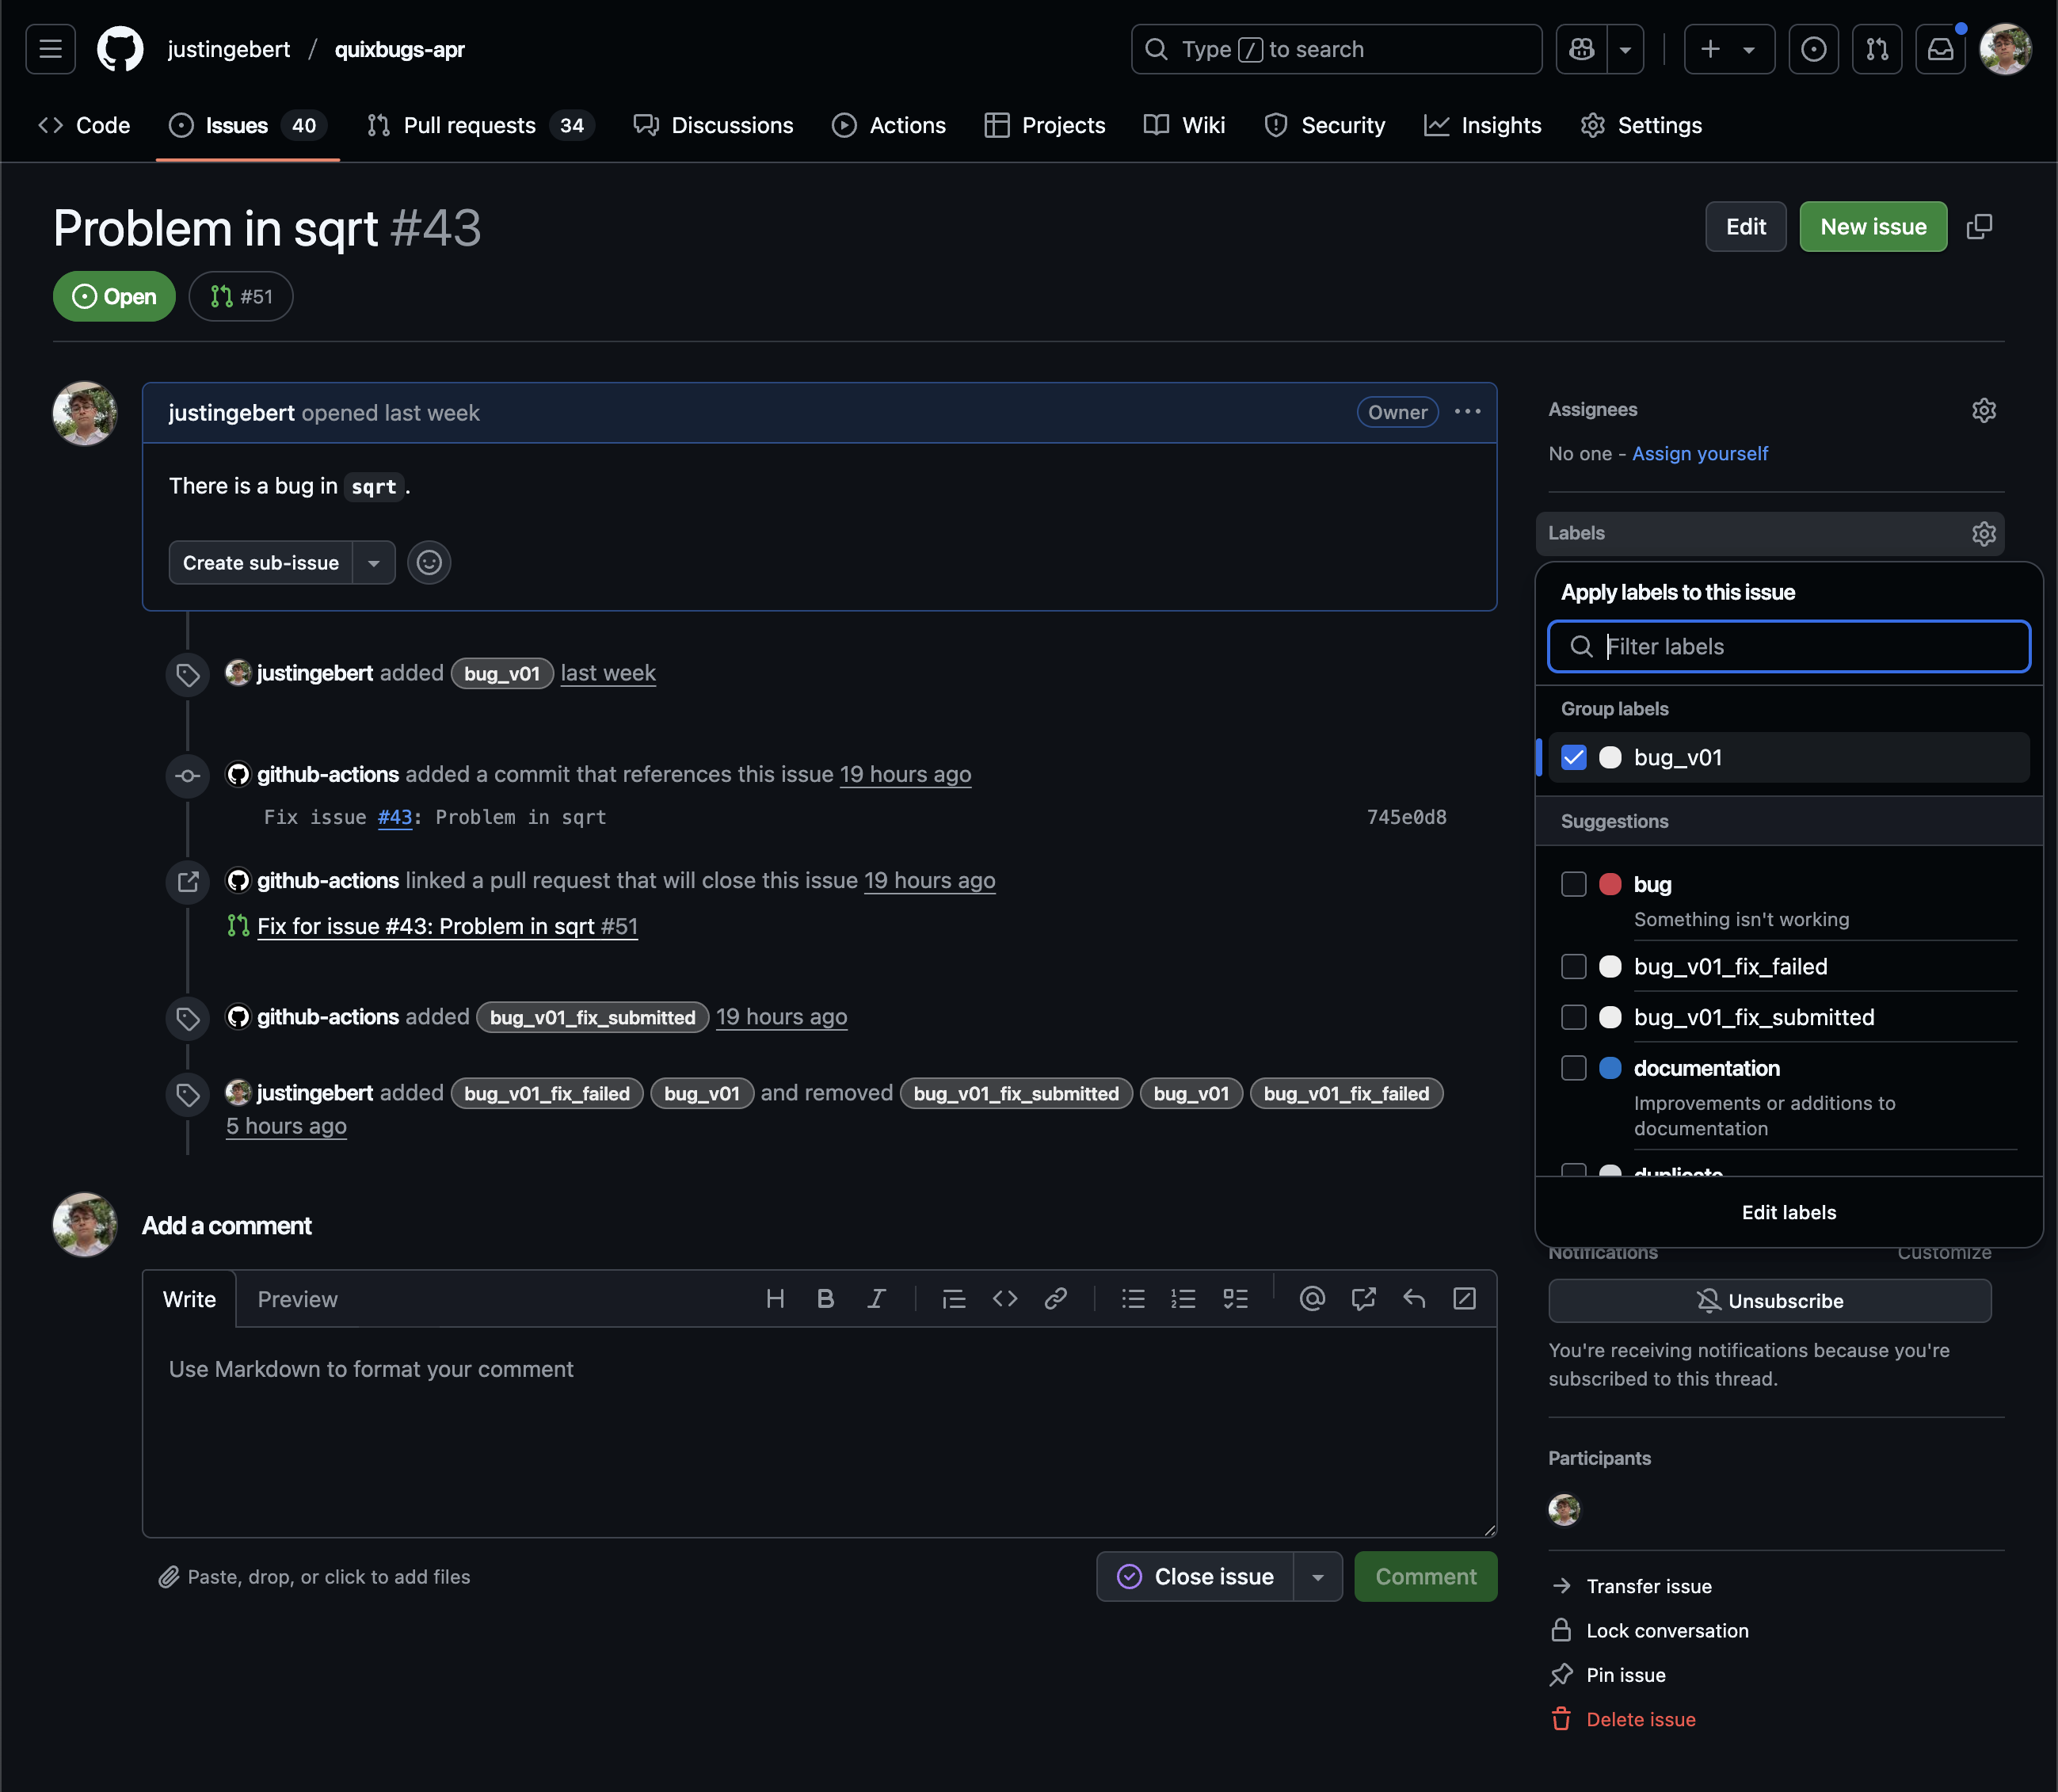
\includegraphics[width=1\textwidth]{images/workflow/label_issue.png}
    \caption{Trigger automatic fixing for single issue}
    \label{fig:issue-trigger}
\end{figure}

The second way collects and processes all issues labeled with the ``bug\_v01'' label by scheduling the workflow to run at a specific time or dispatching it manually (see Figure \ref{fig:dispatch}). This allows for a more controlled approach to bug fixing, where issues are processed in batches.

\begin{figure}[H]
    \centering
    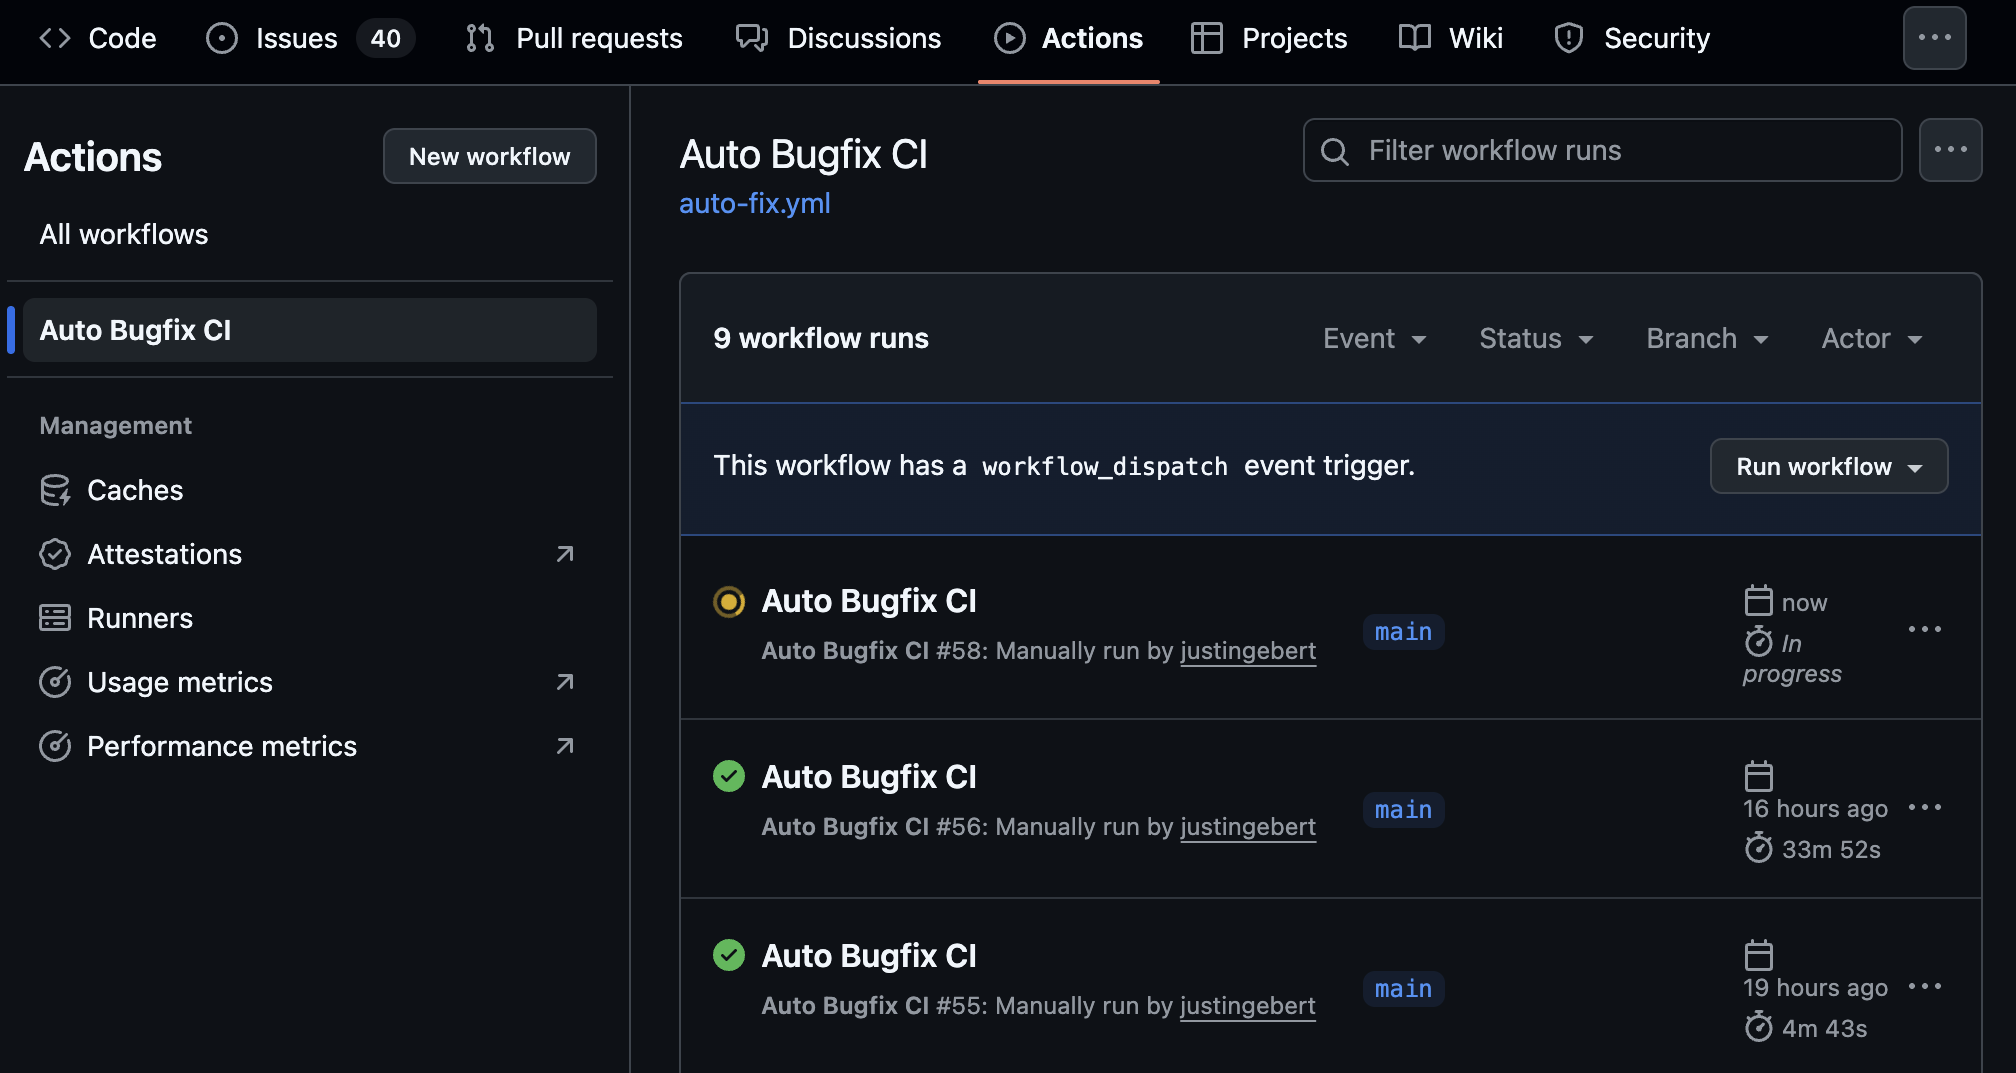
\includegraphics[width=1\textwidth]{images/workflow/manual_dispatch.png}
    \caption{Manual Dispatch of APR}
    \label{fig:dispatch}
\end{figure}

When the workflow is triggered, it creates a new run in the GitHub Actions tab (see Figure \ref{fig:apr-action}). This executes the bug fixing logic described in \ref{chapter:implementation}.

\begin{figure}[H]
    \centering
    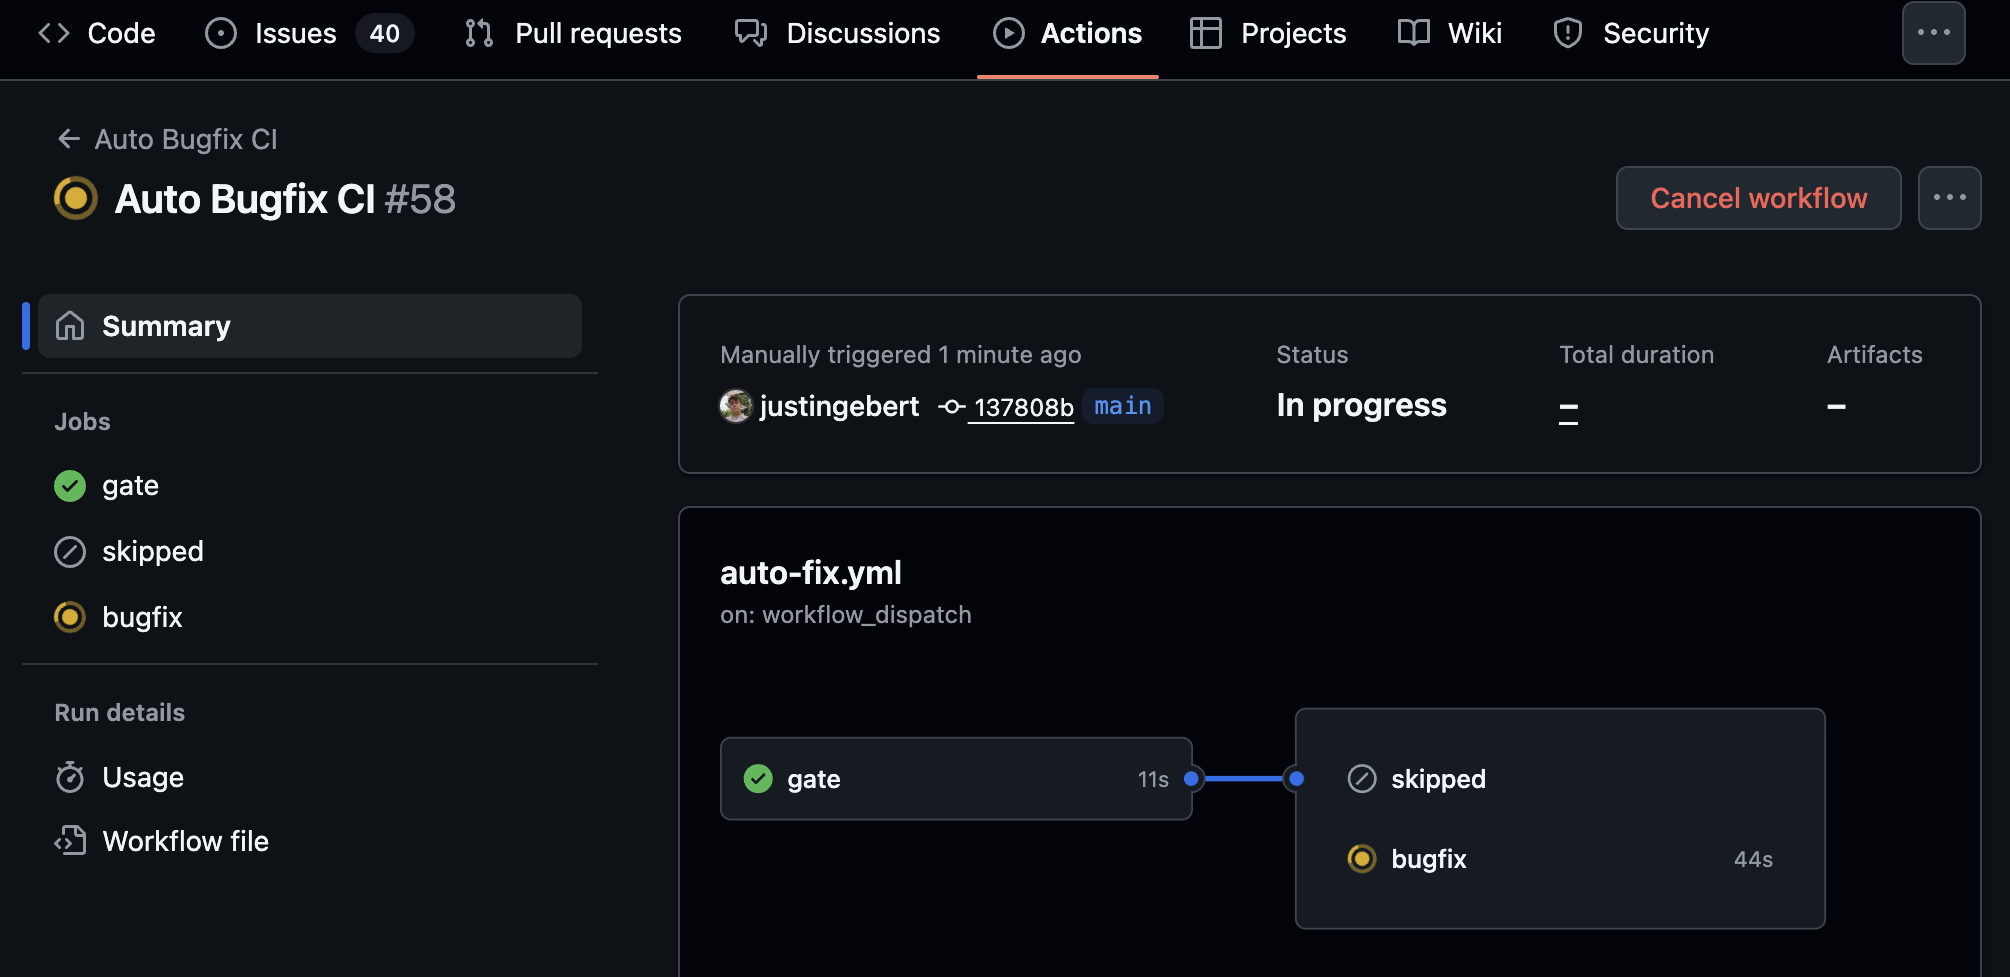
\includegraphics[width=1\textwidth]{images/workflow/new_action.png}
    \caption{GitHub Action Run}
    \label{fig:apr-action}
\end{figure}

A run can produce two possible outcomes for each issue it processes. Firstly, on a successful repair attempt, it creates a Pull Request with the changes made to the codebase and links the issue to it. The created Pull Requests allow code review and merging of the fixed changes into the main branch. When merged, the issue will be automatically closed. Figure \ref{fig:pr} shows an example of a resulting Pull Request created by the APR system.

\begin{figure}[H]
    \centering
    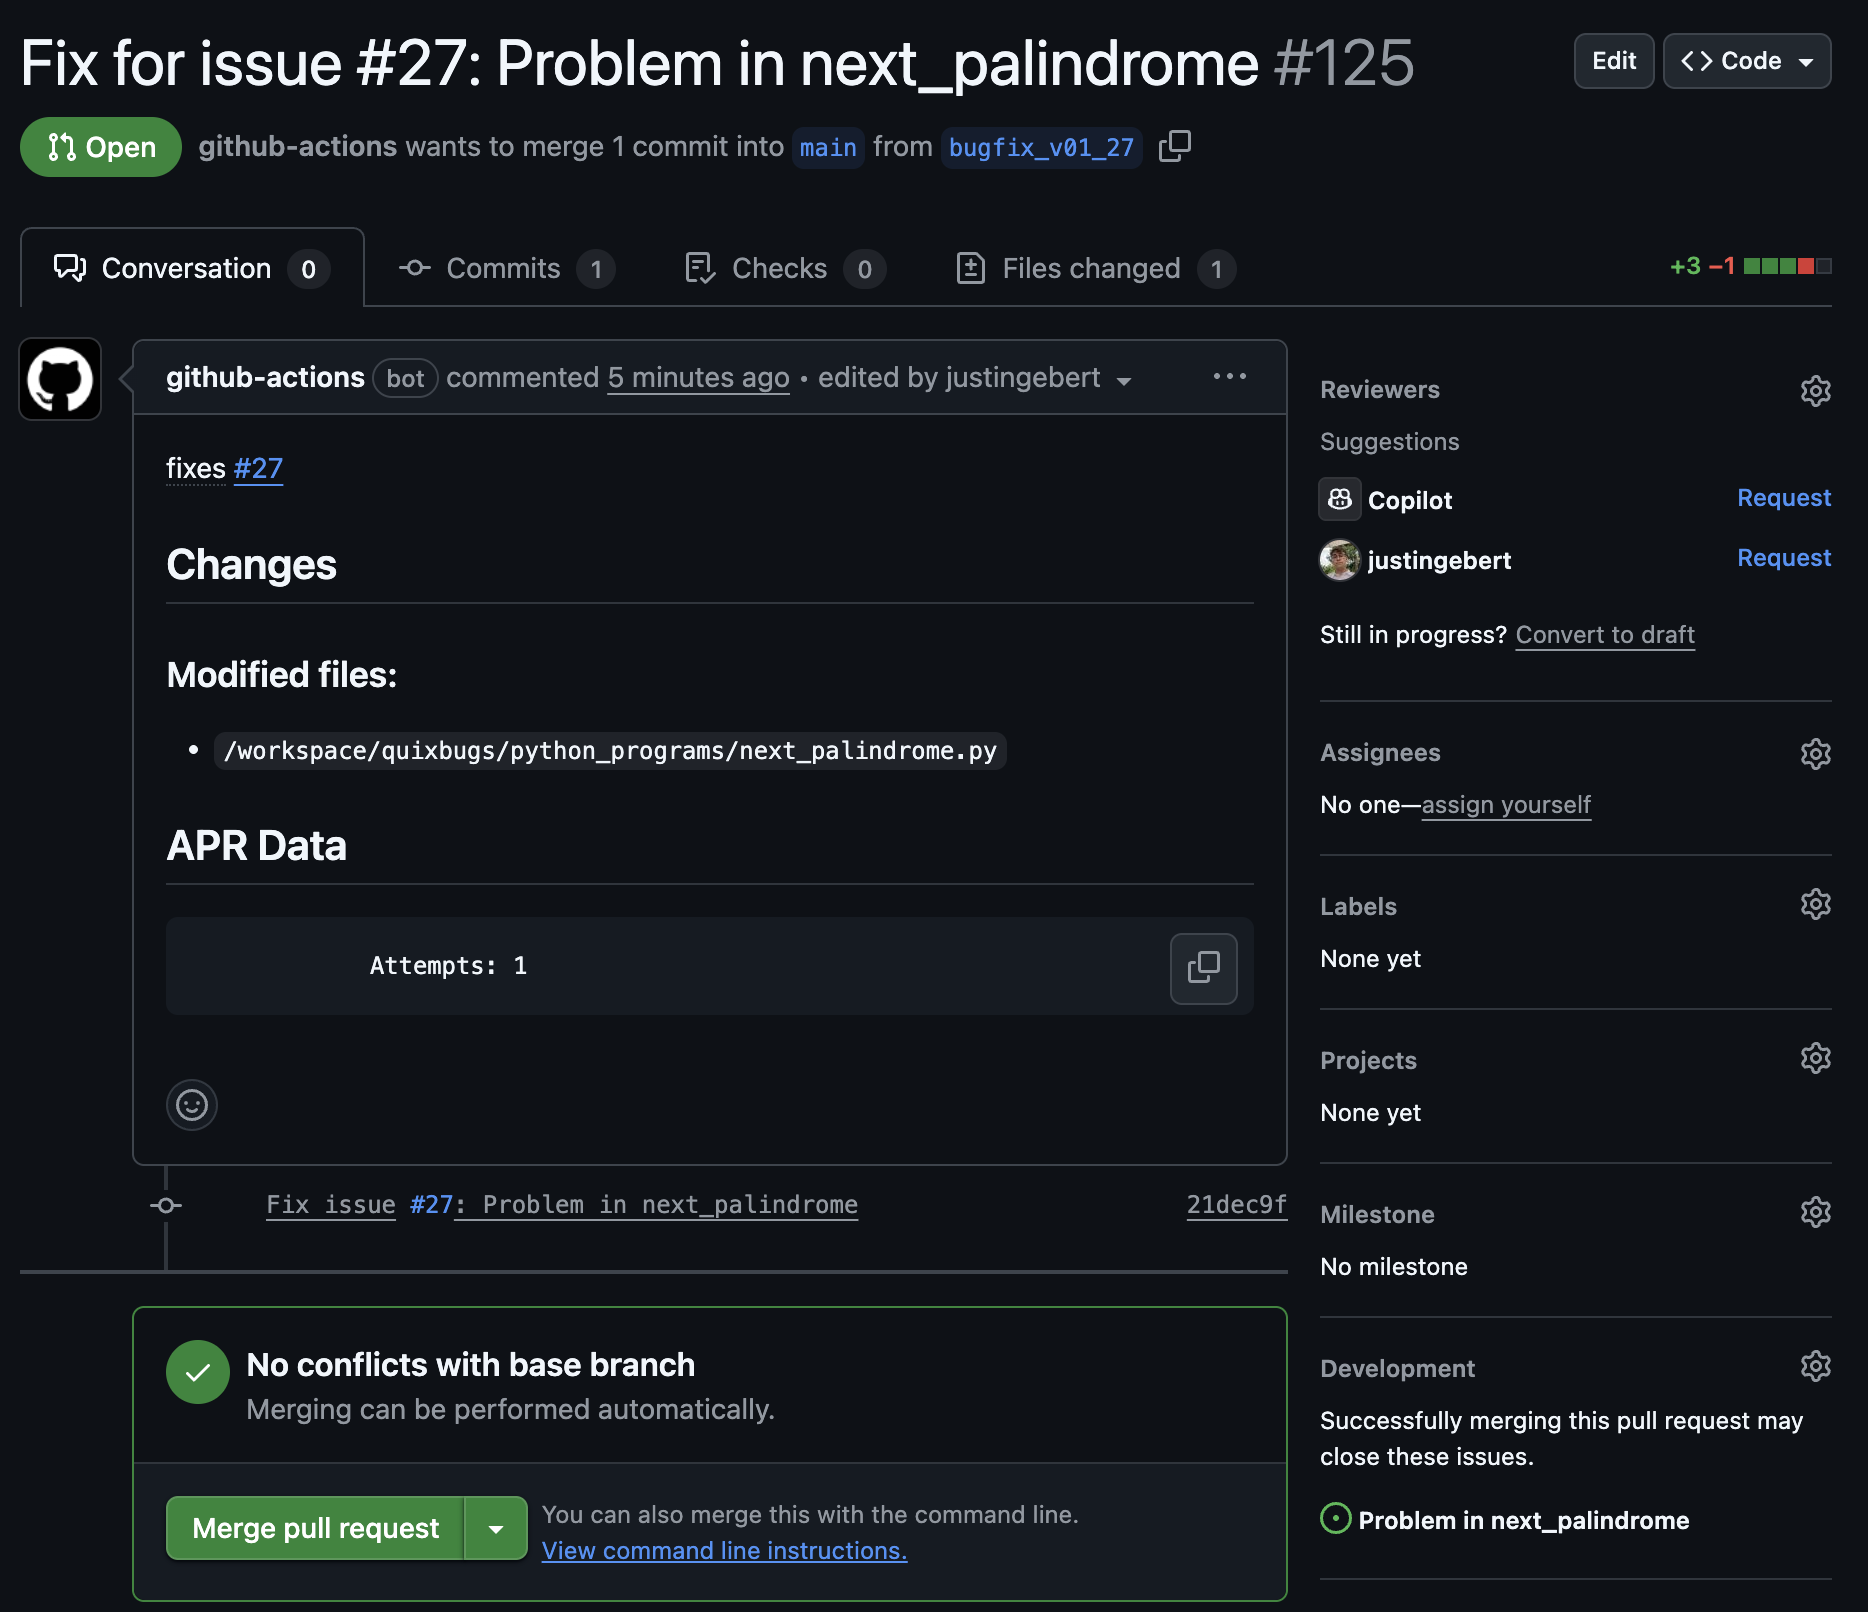
\includegraphics[width=1\textwidth]{images/workflow/pr.png}
    \caption{Resulting Pull Request}
    \label{fig:pr}
\end{figure}

Secondly, when an issue repair fails after all attempts have been exhausted, the failure is reported to the issue as a comment and the issue is labeled as failed (see Figure \ref{fig:failure-report}) so it won't be picked up again. This allows for easy tracking of issues that could not be fixed by the APR system.
\begin{figure}[H]
    \centering
    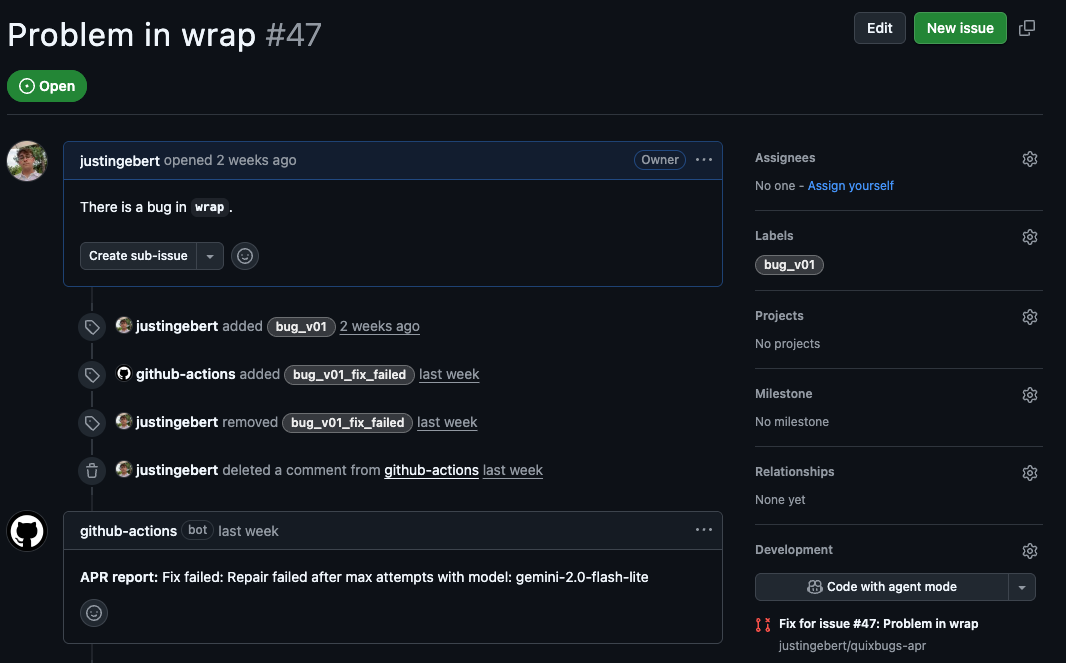
\includegraphics[width=1\textwidth]{images/workflow/failure_comment.png}
    \caption{Failure Report}
    \label{fig:failure-report}
\end{figure}

Failed issues can be picked up again by adding new context to the issue. This can be done by adding a comment to the issue, which will trigger the APR system to pick up the issue again and try to fix it with the new context. This allows for a more dynamic approach to bug fixing, where issues can be fixed as new information becomes available.

%TODO pipeline from comment screenshot

For transparency and debugging, each run provides a live log stream in the GitHub Actions tab (see Figure \ref{fig:log-stream}). This allows users to see the progress of the run and any errors that occur during the execution. For further analysis, logs, metrics, and the complete context are published as artifacts to each run, available to download in the run view.
\begin{figure}[H]
    \centering
    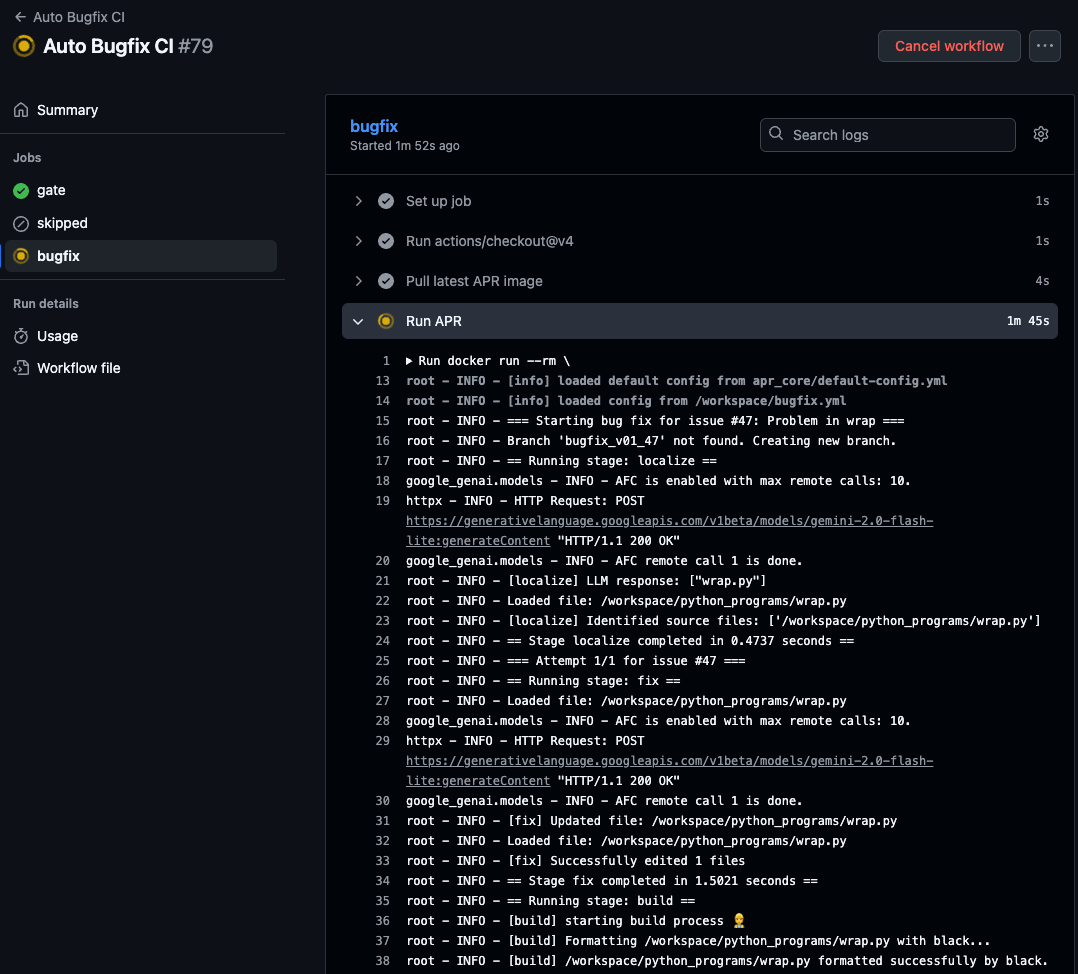
\includegraphics[width=1\textwidth]{images/workflow/logs.png}
    \caption{APR log stream}
    \label{fig:log-stream}
\end{figure}

Figure \ref{fig:flow} visualizes the resulting flow of the APR system. The diagram shows the relation between user actions (yellow) and runs by the integrated APR system.

\begin{figure}[H]
    \centering
    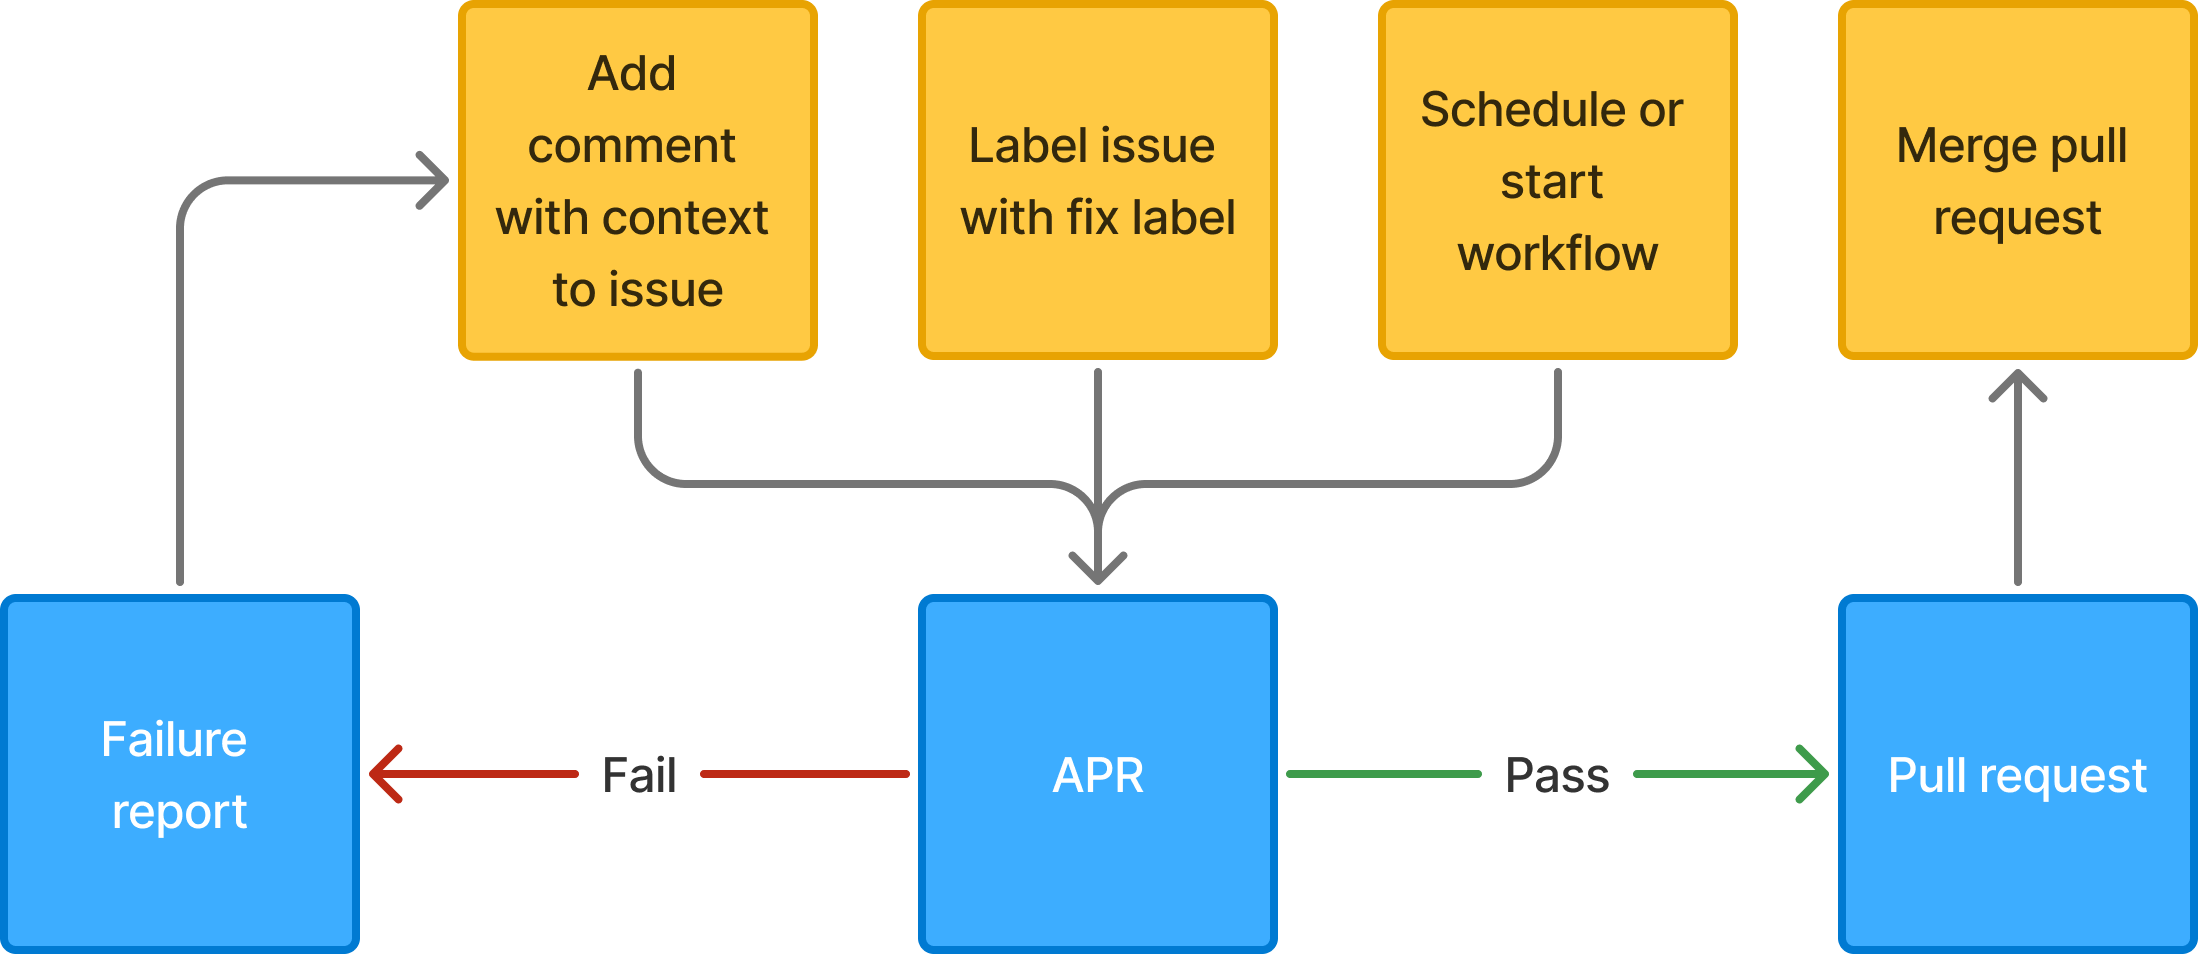
\includegraphics[width=0.9\textwidth]{images/flowcharts/flowresult.png}
    \caption{Resulting flow diagram}
    \label{fig:flow}
\end{figure}

section{Evaluation Results} \label{section:evaluation-results}

In this section, we present the results of the quantitative evaluation of the implemented APR prototype. This evaluation is based on the collected and calculated data for each run of the prototype. How this data was collected and calculated is described in \ref{table:run-metrics}.

\subsection{Validity}

- GitHub runners introduce a lot of computational noise
- Only a small set of runs were performed
- results for average times do not fully ad up to apr core because the timing where stoped when an issue was completed not when the APR core finished 

We asses more threats to validity in section \ref{section:validity}.

\subsection{Baseline of Evaluation}

The resulting data is based on the executions of the APR prototype in the prepared repository (see \ref{subsection:environment-setup}), which contains all 40 issues from the QuixBugs benchmark. For evaluating the effectiveness, performance, and cost, we ran the APR prototype using eleven selected LLM models defined in \ref{subsection:llm-selection}. All models were tested with one attempt per issue to evaluate zero-shot performance and with a retry loop enabled to compare few-shot performance.

\subsection{Results}

The following tables and diagrams show the repair success rate, average cost per issue, and average execution time per issue for each model used in the evaluation. The first table \ref{table:results} shows the results of the evaluation with one attempt per issue, while the second table \ref{table:retry-results} shows the results with the retry loop enabled and the max attempts set to 3.

%TODO add exact model snapshot versions
\begin{table}[H]
    \centering
    \small
    \begin{tabular*}{\textwidth}{@{\extracolsep{\fill}} p{3.5cm} | p{3cm} | p{3cm} | p{3cm} @{}}
        \hline
        \textbf{Model} & \textbf{Repair Success Rate} & \textbf{Average Cost Per Issue} & \textbf{Average Execution Time in seconds} \\
        \hline
        \textbf{gemini-2.0-flash-lite} & 87.5\% & \$0.0001 & 11.33s \\
        \textbf{gemini-2.0-flash} & 87.5\% & \$0.0002 & 8.18s \\
        \textbf{gemini-2.5-flash-lite} & 90.0\% & \$0.0002 & 5.07s \\
        \textbf{gemini-2.5-flash} & 92.5\% & \$0.009 & 20.46s \\
        \textbf{gemini-2.5-pro} & 95.0\% & \$0.07130 & 70.09s \\
        \textbf{gpt-4.1-nano} & 70.0\% & \$0.0001 & 6.73s \\
        \textbf{gpt-4.1-mini} & 90.0\% & \$0.0007 & 8.96s \\
        \textbf{gpt-4.1} & 90.0\% & \$0.0033 & 7.42s  \\
        \textbf{o4-mini} & 90.0\% & \$0.0069 & 23.08s  \\
        \textbf{claude-3-5-haiku} & 0.0\% & \$0.0024 & 9.17s \\
        \textbf{claude-3-7-sonnet} & 87.5\% & \$0.0069 & 11.72s \\
        \textbf{claude-sonnet-4-0} & 90.0\% & \$0.0103 & 12.96s \\
        \hline
    \end{tabular*}
    \caption{Zero shot evaluation results}
    \label{table:results}
\end{table}

\begin{table}[H]
    \centering
    \small
    \begin{tabular*}{\textwidth}{@{\extracolsep{\fill}} p{3.5cm} | p{3cm} | p{3cm} | p{3cm}  @{}}
        \hline
        \textbf{Model} & \textbf{Repair Success Rate} & \textbf{Average Cost}  & \textbf{Average Execution Time} \\
        \hline
        \textbf{gemini-2.0-flash-lite} & 85\% & \$0.0003  & 13.08s \\
        \textbf{gemini-2.0-flash} & 90.0\% & \$0.0004  & 8.27s \\
        \textbf{gemini-2.5-flash-lite} & 90.0\% & \$0.0003 & 7.18s \\
        \textbf{gemini-2.5-flash} & 95.0\% & \$0.0111  & 23.65s \\
        \textbf{gemini-2.5-pro} & 97.5\% & \$0.07086  & 68.78s \\
        \textbf{gpt-4.1-nano} & 90.0\% & \$0.0003  & 10.61s \\
        \textbf{gpt-4.1-mini} & 97.5\% & \$0.0043  & 11.98s \\
        \textbf{gpt-4.1} & 97.5\% & \$0.004 & 7.45s \\
        \textbf{o4-mini} & 100\% & \$0.007  & 21.54s \\
        \textbf{claude-3-5-haiku} & 15.0\% & \$0.0076  & 23.98s \\
        \textbf{claude-3-7-sonnet} & 95.0\% & \$0.0085 & 27.16s \\
        \textbf{claude-sonnet-4-0} & 92.5\% & \$0.0117 & 16.80s \\
        \hline
    \end{tabular*}
    \caption{Few shot evaluation results}
    \label{table:retry-results}
\end{table}

\begin{figure}[H]
    \centering
    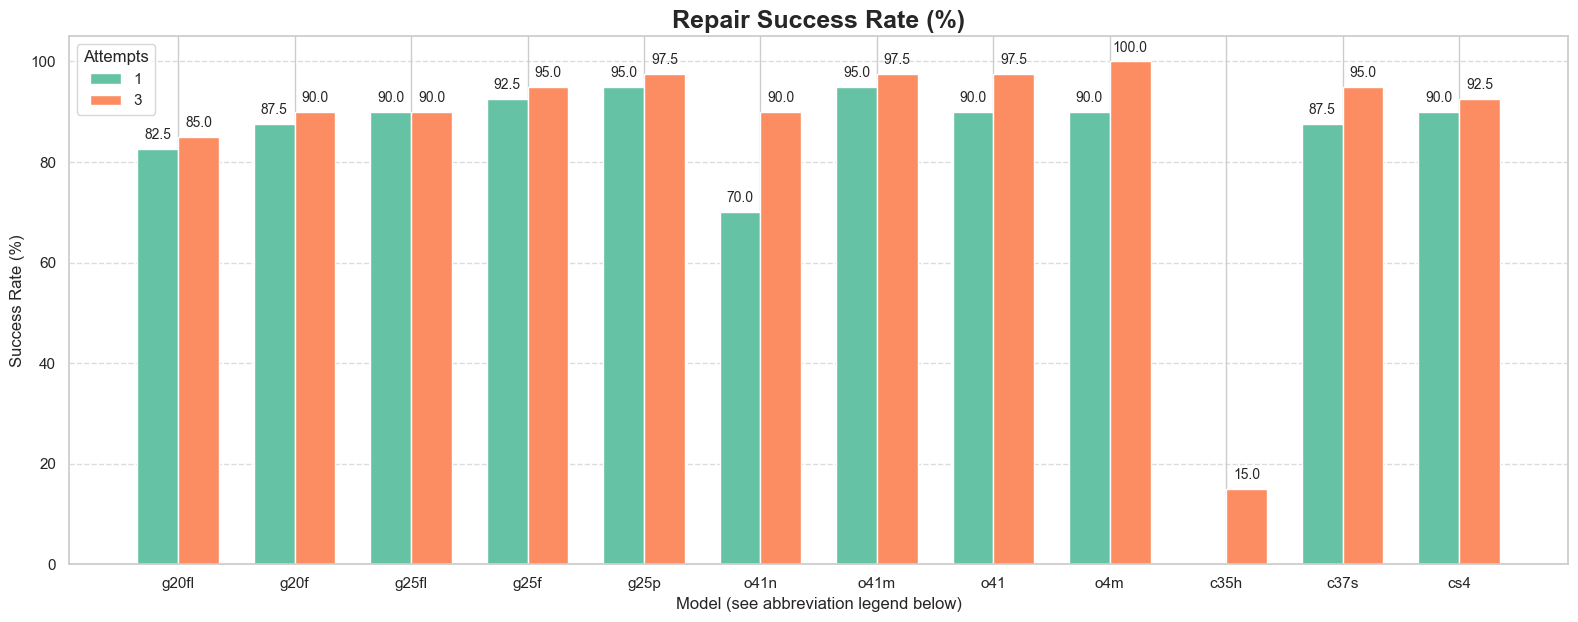
\includegraphics[width=1\textwidth]{images/diagrams/repair_success_rate_per_model_grouped.png}
    \caption{Repair Success Rate per Model}
    \label{fig:repair-success-rate}
\end{figure}

\begin{figure}[H]
    \centering
    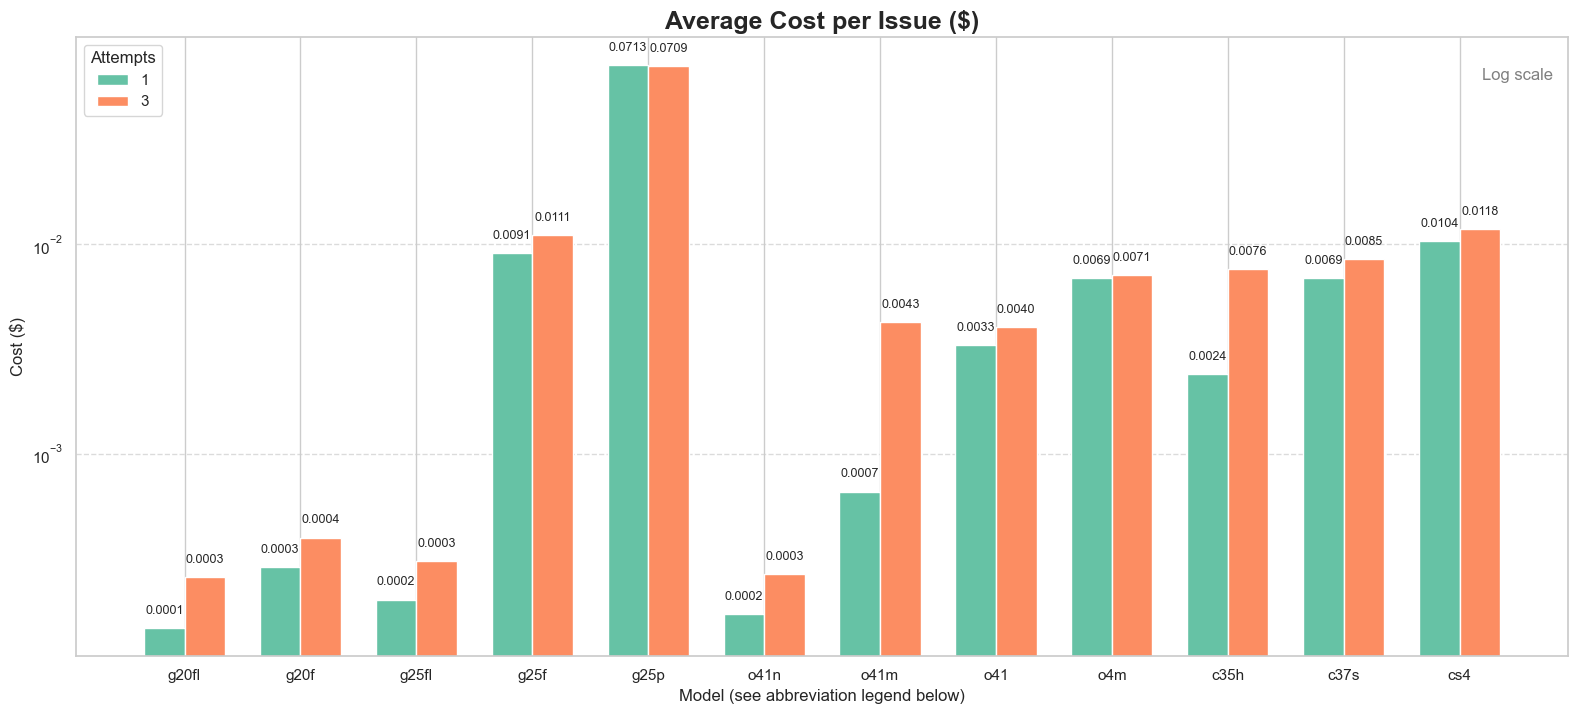
\includegraphics[width=1\textwidth]{images/diagrams/avg_cost_per_issue_per_model_grouped.png}
    \caption{Average Cost per Issue per Model}
    \label{fig:avg-cost-per-issue}
\end{figure}

\begin{figure}[H]
    \centering
    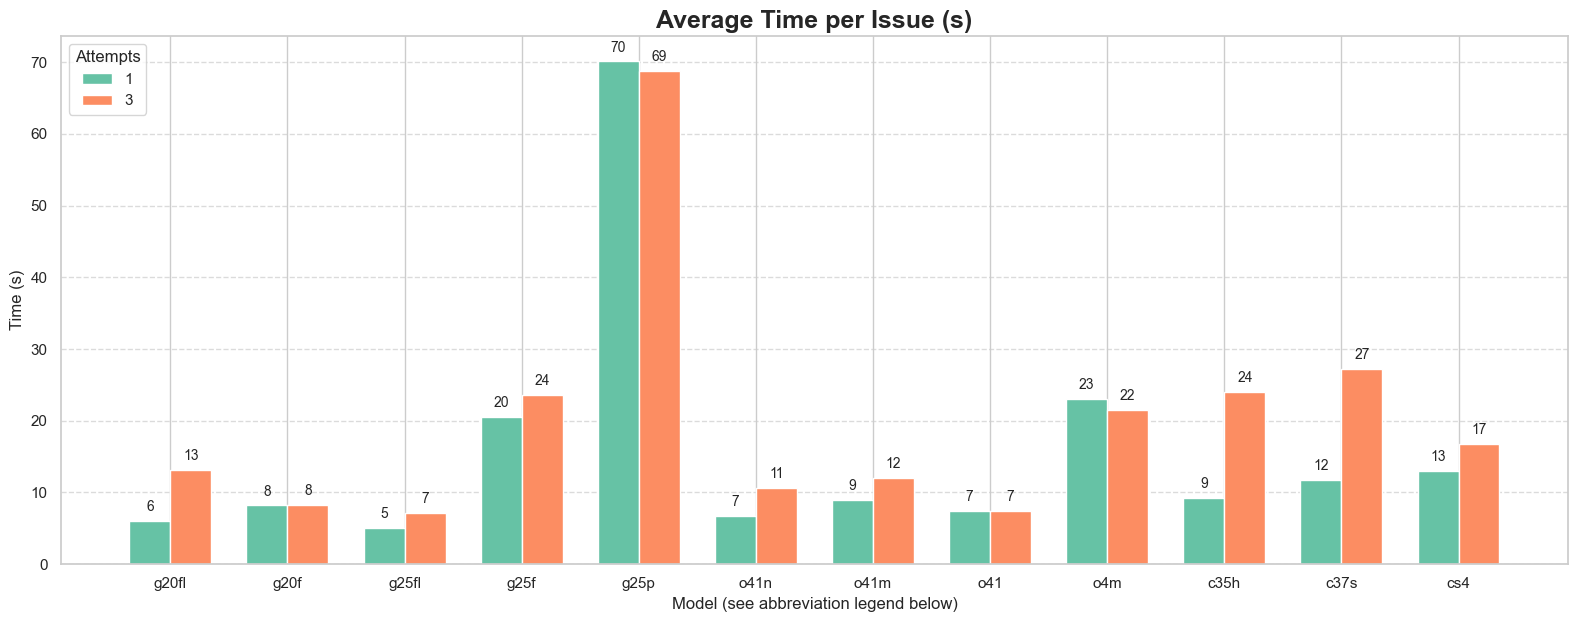
\includegraphics[width=1\textwidth]{images/diagrams/avg_execution_time_per_issue_per_model_grouped.png}
    \caption{Average Execution Time per Issue per Model}
    \label{fig:avg-execution-time-per-issue}
\end{figure}


CI Overhead
\begin{figure}[H]
    \centering
    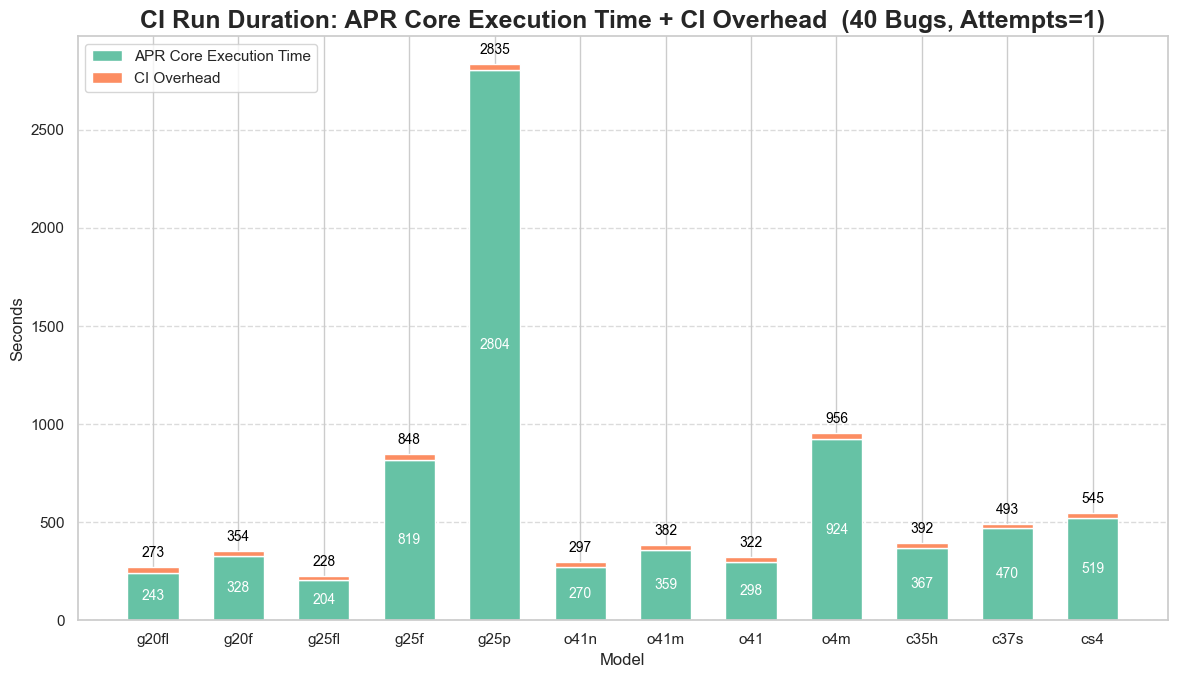
\includegraphics[width=1\textwidth]{images/diagrams/ci_vs_exec_time_per_run_stacked_attempts_1.png}
    \caption{CI Overhead per Run with 1 Attempt}
    \label{fig:ci-vs-exec-time-per-run-attempts-1}
\end{figure}

\begin{figure}[H]
    \centering
    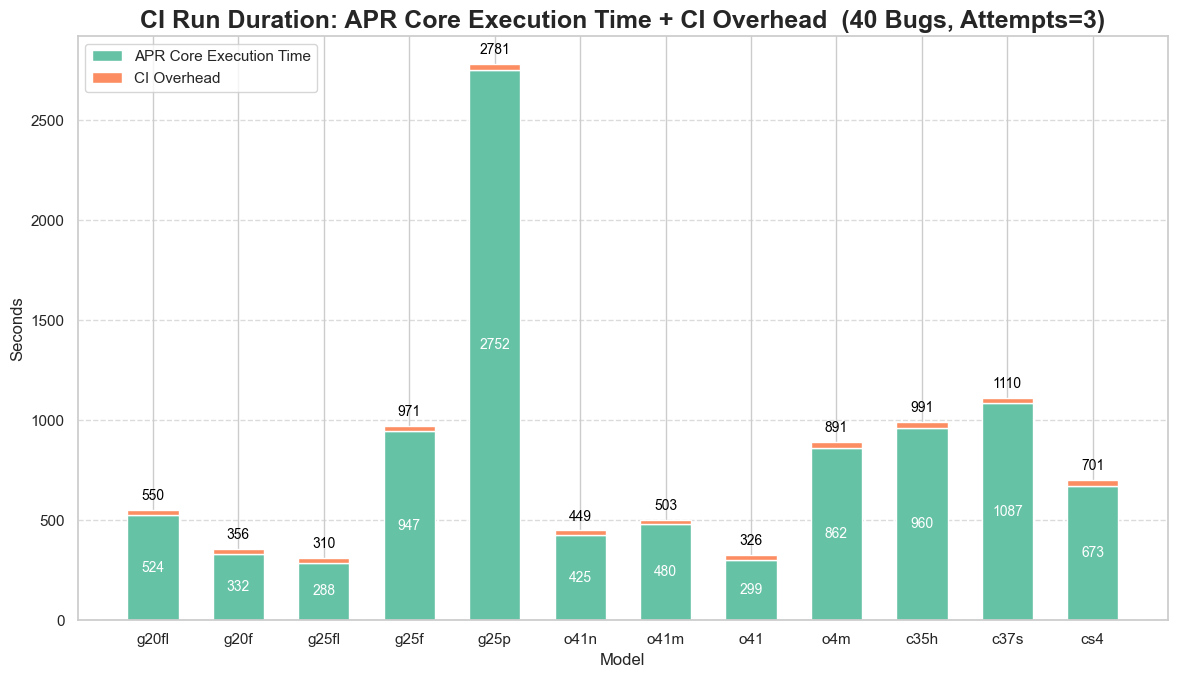
\includegraphics[width=1\textwidth]{images/diagrams/ci_vs_exec_time_per_run_stacked_attempts_3.png}
    \caption{CI Overhead per Run with 3 Attempts}
    \label{fig:ci-vs-exec-time-per-run-attempts-3}
\end{figure}


The full set of resulting data can be found in the ``apr\_evaluation'' directory of the quixbugs-apr repository, listed in the Appendix \ref{chapter:appendix}.